\documentclass[11pt)]{beamer}
\usetheme{Copenhagen}

\defbeamertemplate*{headline}{split}
{%
  \leavevmode%
  \hbox{%
  \begin{beamercolorbox}[wd=.5\paperwidth,ht=2.65ex,dp=1.5ex,right]{section in head/foot}%
    \usebeamerfont{section in head/foot}\insertsectionhead\hspace*{2ex}
  \end{beamercolorbox}%
  \begin{beamercolorbox}[wd=.5\paperwidth,ht=2.65ex,dp=1.5ex,left]{subsection in head/foot}%
    \usebeamerfont{subsection in head/foot}\hspace*{2ex}\insertsubsectionhead
  \end{beamercolorbox}}%
  \vskip0pt%
}

\defbeamertemplate*{footline}{split}
{
	\leavevmode%
   	\hbox{%
      \begin{beamercolorbox}[wd=.5\paperwidth,ht=2.25ex,dp=1ex,center]{author in head/foot}%
        \usebeamerfont{author in head/foot}\insertshortauthor
      \end{beamercolorbox}%
      \begin{beamercolorbox}[wd=.4\paperwidth,ht=2.25ex,dp=1ex,center]{title in head/foot}%
        \usebeamerfont{title in head/foot}\insertshorttitle
      \end{beamercolorbox}%
      \begin{beamercolorbox}[wd=.1\paperwidth,ht=2.25ex,dp=1ex,right]{date in head/foot}%
        \usebeamerfont{date in head/foot}
        \insertframenumber{} / \inserttotalframenumber\hspace*{2ex}
      \end{beamercolorbox}}%
      \vskip0pt%
}

\setbeamertemplate{caption}{\raggedright\insertcaption\par}



\usepackage[utf8]{inputenc}
\usepackage{amsmath}
\usepackage{amsfonts}
\usepackage{amssymb}
\usepackage{graphicx}
\usepackage{lmodern}
\usepackage{multirow}
\graphicspath{ {./figures/} }
\author{Judith Abécassis, Timothée Lacroix}
\title{SSL via Locally Sensitive Hashing (LSH)}
%\setbeamercovered{transparent} 
\setbeamertemplate{navigation symbols}{} 
%\logo{} 
\institute{Graphs in Machine Learning} 
\date{April 2015} 
%\subject{}
\AtBeginSection[]

\usepackage{tikz}
\usetikzlibrary{shapes,arrows,positioning}

\begin{document}

\begin{frame}
\titlepage
\end{frame}

{
  \begin{frame}
    \frametitle{Table of contents}
    \tableofcontents[currentsection]
  \end{frame}
}


\section{Challenge}
\begin{frame}{Classify a lot of elements in a SSL context}

		\begin{figure}[ht]
			\centering
			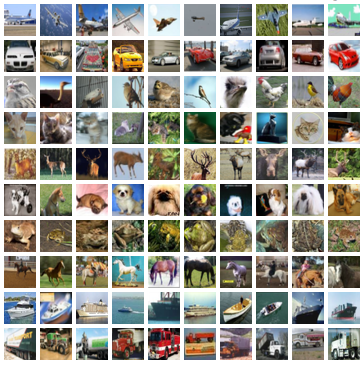
\includegraphics[width=\textwidth]{cifar-10.png}
			\caption{Crowd}
		\end{figure}


\end{frame}

\section{Semi-Supervised Learning Framework}
\begin{frame}{Leverage information from unlabeled nodes in the graph}

\end{frame}

\begin{frame}{The harmonic solution}
\end{frame}

\begin{frame}{Issues arise with the size of the graph}
\end{frame}

\section{Locality Sensitive Hashing}
\begin{frame}{Presentation of the principle}
\end{frame}

\begin{frame}{Accuracy}
\end{frame}

\section{Theory}
\begin{frame}{}
\end{frame}

\begin{frame}{Limitations to obtaining a bound for LSH}
\end{frame}

\begin{frame}{Empirical results on LSH accuracy}
\end{frame}

\section{Experiments}
\begin{frame}{The tinyImage dataset and preprocessing steps}
\end{frame}

\begin{frame}{Setting to assess performance}
\end{frame}

\begin{frame}{Problems with LSH and GRaphlab implementations}
\end{frame}

\begin{frame}{Results}
\end{frame}

\section{Conclusion}
\begin{frame}{Conclusion}
\end{frame}

\begin{frame}{Future work}
\end{frame}











\end{document}